% % % % % % % % % % % % % % % % % % % % % % % % % % % % % % % % % % % % % % % % %
% INTRO
% % % % % % % % % % % % % % % % % % % % % % % % % % % % % % % % % % % % % % % % %
\section{Time box 7}
\listoftodos
\subsection{Time box planning}

\begin{figure}[H]
	\begin{centering}
		\missingfigure{Updated timebox figure}
		%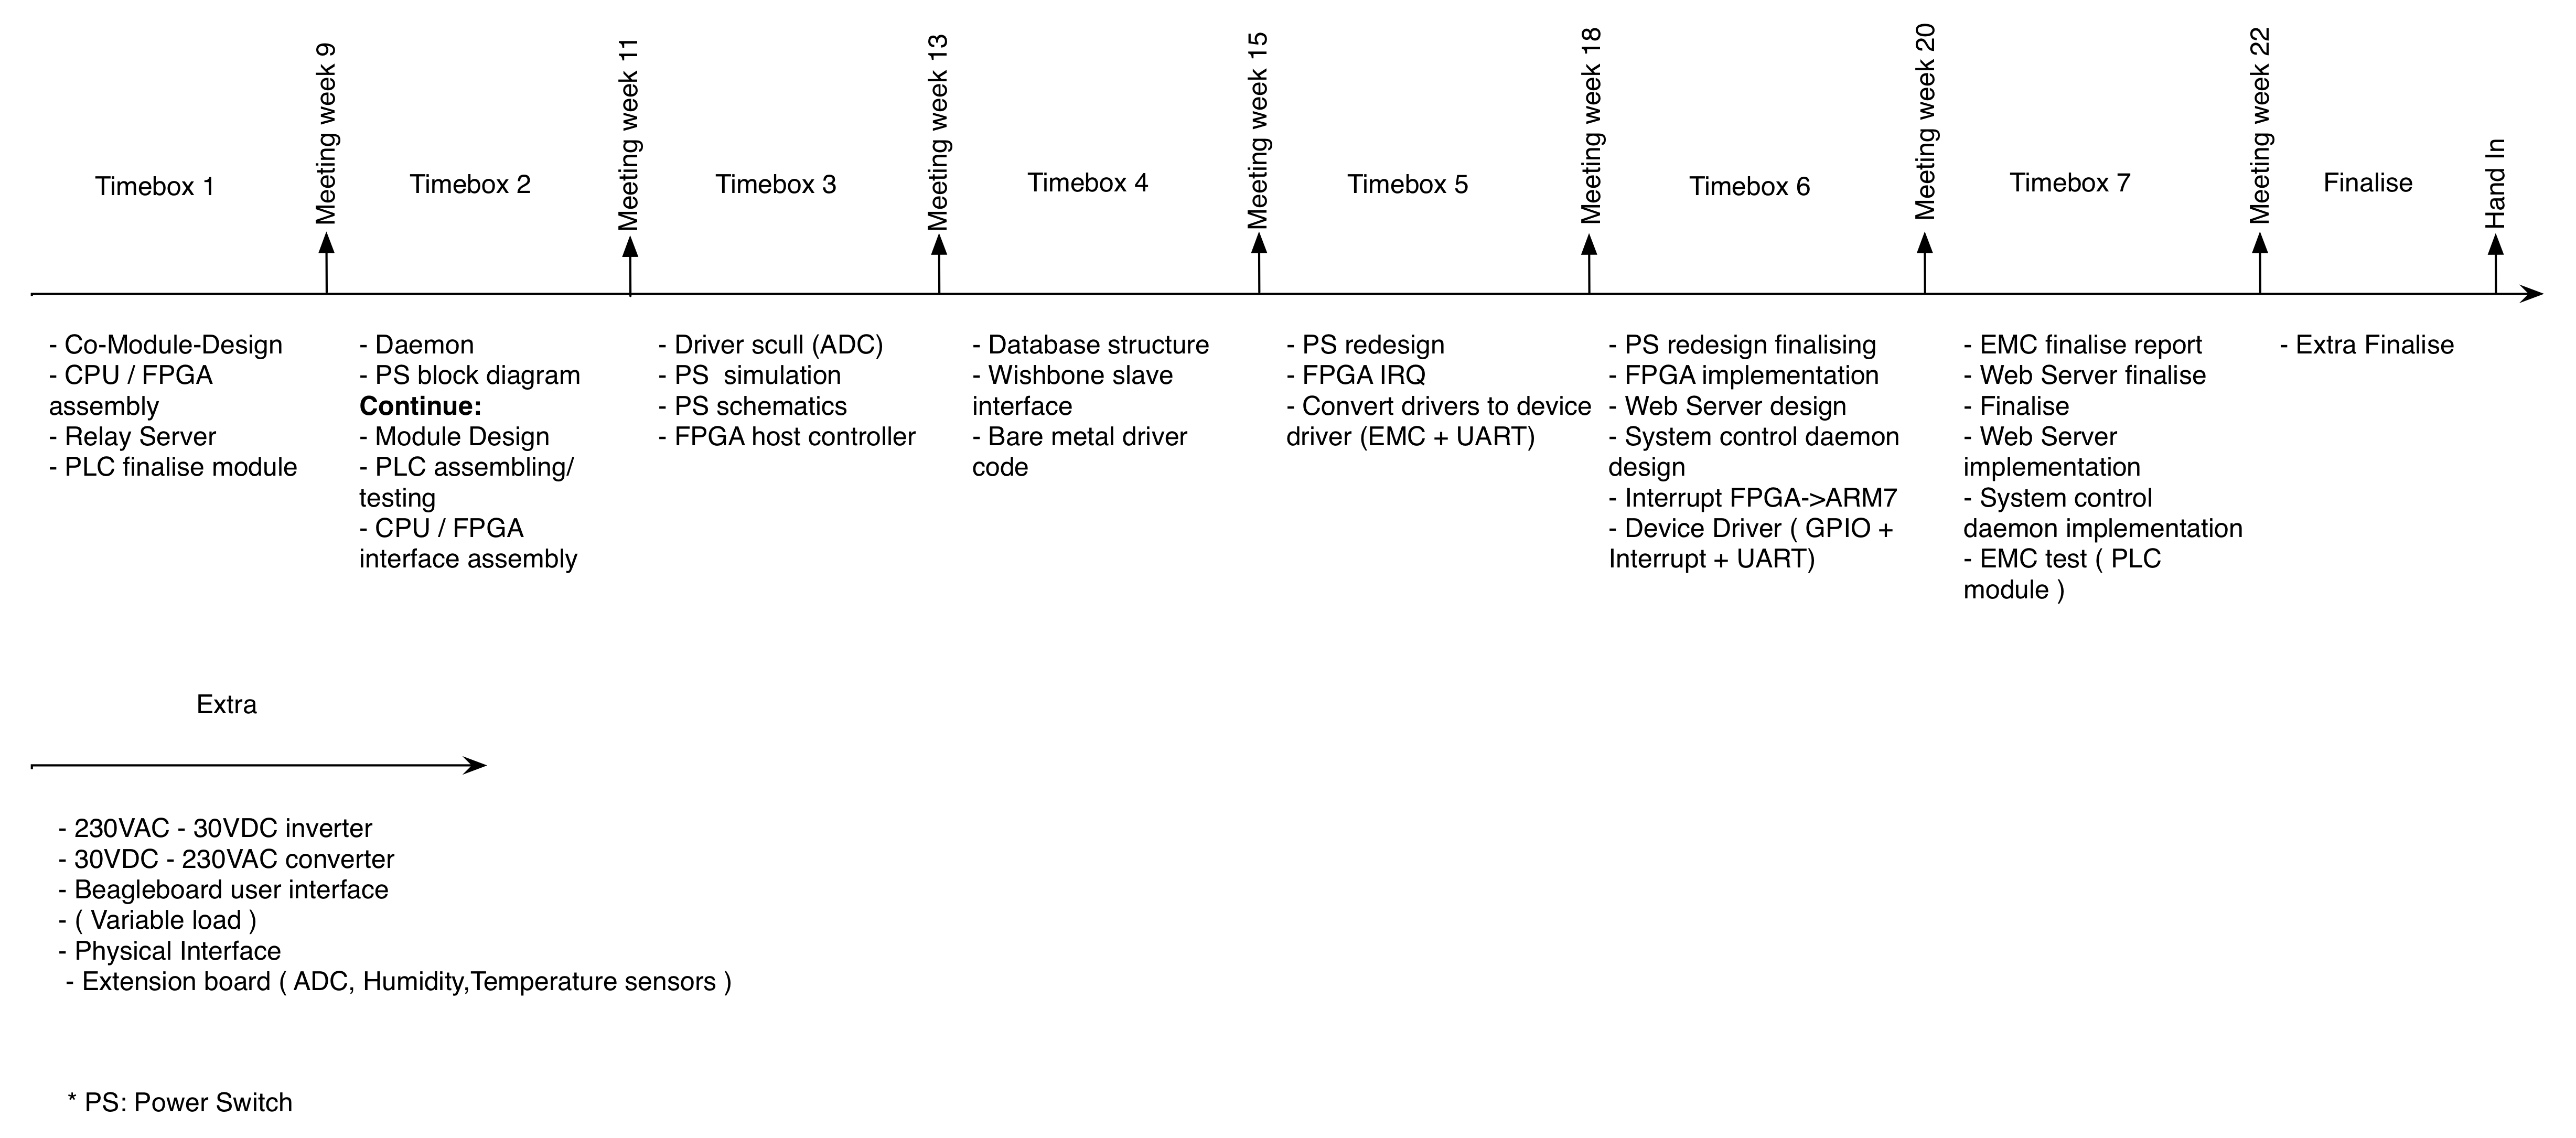
\includegraphics[width=1.0\textwidth]{images/tb_r5.png}
		%\caption{Updated time-box}
	\end{centering}
\end{figure}

\subsubsection{Work to be done in this time box}
\todo[inline]{Update List}
\begin{itemize}
	\item Theis thing
	\begin{itemize}
		\item Sub thing
	\end{itemize}
	\item Jesus thing
		\begin{itemize}
			\item sub thing
		\end{itemize}
	\item Dennis thing
	\begin{itemize}
		\item Sub thing
	\end{itemize}
\end{itemize}

\paragraph{Description:}
\todo[inline]{Update Description}
\begin{description}
	\item[Theis thing]
	\item[Jesus thing]
	\item[Dennis thing]
\end{description}

\subsubsection{Time planning}

\begin{table}[H]
\centering
	\todo[inline]{Update Time}
	\begin{tabular}{|l|c|c|c|c|c|}
		\hline
		~			& Theis thing			& Jesus thing		& Dennis thing	\\ \hline
		Estimation	& xx					& xx				& xx			\\
		Actual		& xx					& xx				& xx			\\
		Developer	& Theis					& Paulo				& Dennis		\\
		\hline
	\end{tabular}
	\caption{Estimation and actual time used on the project}
\end{table}
% % % % % % % % % % % % % % % % % % % % % % % % % % % % % % % % % % % % % % % % %
% % % % % % % % % % % % % % % % % % % % % % % % % % % % % % % % % % % % % % % % %
% Theis Thing
% % % % % % % % % % % % % % % % % % % % % % % % % % % % % % % % % % % % % % % % %
\subsection{Theis thing - Theis}
%			Intro
%					verification specification
%					deployment specification
%
\subsubsection{Analysis}
%			Analysis
%
%                Refactored block diagram
%                Refactored class diagram
%                Detailed use cases
%                User interface specification
%                System interface specification
%                Dimensioning specification 
%
\subsubsection{Design}
%       	 Design
%
%                UML/SysML deployment view(s)
%                Mechanical specifications and dimensioning
%                HW module specification per block
%                UML SW deployment view
%                Class specification
%                Refactored class diagram
%                Use case scenarios specifications
%                Sequence diagrams
%
\subsubsection{Implementation}
%     	   Implementation
%
%                Mechanical drawings with details explained
%                Electronic diagrams with details explained
%                Source code with details explained
%                Description of integration 
%
\subsubsection{Verification}
%       	 Verification
%
%                Module tests
%                Integration tests
%                Acceptance test
\subsubsection{Conclusion}
% % % % % % % % % % % % % % % % % % % % % % % % % % % % % % % % % % % % % % % % %
% % % % % % % % % % % % % % % % % % % % % % % % % % % % % % % % % % % % % % % % %
% Jesus Thing
% % % % % % % % % % % % % % % % % % % % % % % % % % % % % % % % % % % % % % % % %
\subsection{Jesus thing - Paulo}
%			Intro
%					verification specification
%					deployment specification
%
\subsubsection{Analysis}
%			Analysis
%
%                Refactored block diagram
%                Refactored class diagram
%                Detailed use cases
%                User interface specification
%                System interface specification
%                Dimensioning specification 
%
\subsubsection{Design}
%       	 Design
%
%                UML/SysML deployment view(s)
%                Mechanical specifications and dimensioning
%                HW module specification per block
%                UML SW deployment view
%                Class specification
%                Refactored class diagram
%                Use case scenarios specifications
%                Sequence diagrams
%
\subsubsection{Implementation}
%     	   Implementation
%
%                Mechanical drawings with details explained
%                Electronic diagrams with details explained
%                Source code with details explained
%                Description of integration 
%
\subsubsection{Verification}
%       	 Verification
%
%                Module tests
%                Integration tests
%                Acceptance test
\subsubsection{Conclusion}
% % % % % % % % % % % % % % % % % % % % % % % % % % % % % % % % % % % % % % % % %
% % % % % % % % % % % % % % % % % % % % % % % % % % % % % % % % % % % % % % % % %
% Dennis Thing
% % % % % % % % % % % % % % % % % % % % % % % % % % % % % % % % % % % % % % % % %
\subsection{Dennis thing - Dennis}
%			Intro
%					verification specification
%					deployment specification
%
\subsubsection{Analysis}
%			Analysis
%
%                Refactored block diagram
%                Refactored class diagram
%                Detailed use cases
%                User interface specification
%                System interface specification
%                Dimensioning specification 
%
\subsubsection{Design}
%       	 Design
%
%                UML/SysML deployment view(s)
%                Mechanical specifications and dimensioning
%                HW module specification per block
%                UML SW deployment view
%                Class specification
%                Refactored class diagram
%                Use case scenarios specifications
%                Sequence diagrams
%
\subsubsection{Implementation}
%     	   Implementation
%
%                Mechanical drawings with details explained
%                Electronic diagrams with details explained
%                Source code with details explained
%                Description of integration 
%
\subsubsection{Verification}
%       	 Verification
%
%                Module tests
%                Integration tests
%                Acceptance test
\subsubsection{Conclusion}
% % % % % % % % % % % % % % % % % % % % % % % % % % % % % % % % % % % % % % % % %
% % % % % % % % % % % % % % % % % % % % % % % % % % % % % % % % % % % % % % % % %
% Deployment
% % % % % % % % % % % % % % % % % % % % % % % % % % % % % % % % % % % % % % % % %
\subsection{Deployment}
	%which versions of the prototype the customer will get
	%with what functionality.
\paragraph{Theis thing}
%
%
\paragraph{Jesus thing}
%
%
\paragraph{Dennis thing}
%
%